\documentclass[12pt, A4]{report}

\usepackage{graphicx}
\graphicspath{{./images/}}

\usepackage{hyperref}
\hypersetup{
    colorlinks=true,
    linkcolor=blue,
    filecolor=magenta,      
    urlcolor=cyan,
}

\urlstyle{same}


\title{\textbf{Decesion Tree}}
\author{Sahasra Ranjan}
\date{April 2020}

\begin{document}

\begin{titlepage}
\maketitle
\end{titlepage}

A decesion tree is a map of the possible outcomes of a series of a related choices. It allows to weigh possible actions against one another based of various factors.\par
It uses a tree-like model of decesion. It typically starts with a single node, which branches into possible outcomes. Each of those outcomes leads to additional nodes, which branch off into other possiblities. 

\begin{figure}[h]
	\centering
	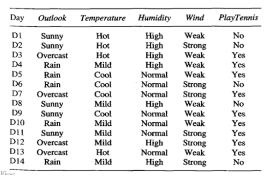
\includegraphics[width=6cm, height=4cm]{dtdata1.png}
	\caption{Dataset for possiblity of a tennis match}
	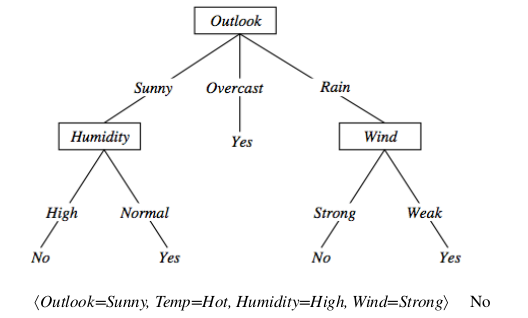
\includegraphics[width=8cm, height=5cm]{dtdata2.png}
	\caption{Decesion Tree for the same}
\end{figure}

\subsection*{Advantages and Disadvantages of Decesion Trees}
	\textbf{Advantages:}
	\begin{itemize}
		\item Performs classification without requiring much computation.
		\item Provides clear indication of important fields for prediction of classification.
	\end{itemize}
	\vspace{15mm}
	\textbf{Disadvantages:}
	\begin{itemize}
		\item Less appropriate for predicting continious attributes.
		\item Computationally expensive to train
	\end{itemize}

\vspace{5mm}
\subsection*{Creating a Decesion Tree}
	For every node, we have to create subtrees with all the possiblities. and then further repeat for other features.\par
	For eg., In the tennis match problem, for the first node  let's check outlook, since having three possiblity (viz. Sunny, Overcast, Rainy), we created three subtrees and then further we keep asking for other features like Humidity \& wind to get the final tree.  

\vspace{5mm}
\subsection*{Greedy Approach for creating decesion tree}
	Greedy approach is implemented by making an optimal local choice at each node. By making these local optimal choices, we reach the approximate optimal solution globaly.

	The algorithm can be summarized as: 
	\begin{enumerate}
		\item At each stage (node), pick out the best feature as the test conditiion.
		\item Now split the node into possibel outcomes (internal nodes)
		\item Repeat the above steps till all the test conditions have been exhausted into leaf nodes.
	\end{enumerate}

\vspace{5mm}
\subsection*{Continuous Features}
	There might be some feature which are not categorical, for these we need to create possibilities on the basis of aprropriate ranges. One such tree is shown below:
	\begin{figure}[h]
		\centering
		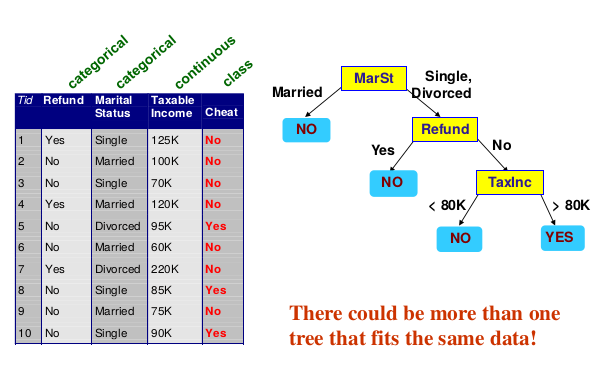
\includegraphics[width=12cm, height=6cm]{continuousDT.png}
		\caption{Decesion tree with continuous feature}
	\end{figure}


\subsection*{Entropy}
	In the most layman terms, Entropy is nothing but the \textbf{The measure of disorder}.
	Why is it important to study entropy for machine learning? \\
	\\ Entropy is a measure of disorder or uncertainity and the goal of machine learning models and Data Scientists in general is to reduce uncertainity.\\
	\\ The Mathematical formula for entropy is - 
	\begin{equation}\label {eq:entropy}
		E(S) = \sum_{i=1}^c - p_i log_2 p_i\
	\end{equation}
	Where $p_i$ is the frequentist probability of an element/class $i$ in out data.\\
	\\ Let's say we have only two classes, a positive and a negative class. Out of 100 data, suppose that 70 belongs to $-$ve class and 30 to $+$ve. Then, P$+$ will be 0.3 and P$-$ will be 0.7.
	\vspace{4mm}
	Entropy $E$ will be given by:
	\begin{equation}
		E = -\frac{3}{10} \times log_2{\frac{3}{10}}-\frac{7}{10} \times log_2{\frac{7}{10}} \approx \textbf{0.88}
	\end{equation}
	\begin{figure}[h]
		\centering
		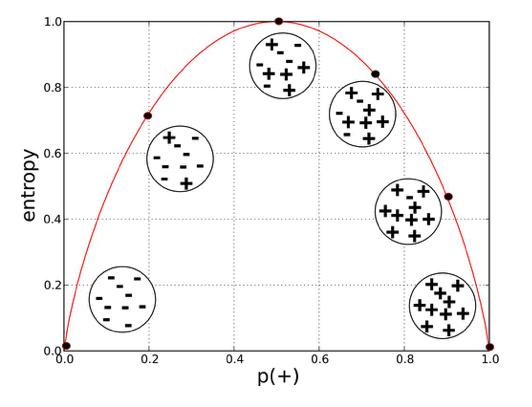
\includegraphics[width=8cm, height=6cm]{entropyDT.png}
		\caption{Entropy distribution frequentist probability}
	\end{figure}

\subsection*{Information Gain}
	Information gain is basically how much Entropy is removed after training a decesion tree.\\
	\textbf{Higher information gain = more entropy removed.}\\
	In technical terms, Information Gain from X on Y is defined as:
	\begin{equation}\label{eq:inforamtion gain}
		IG(Y,X) = E(Y) - E(Y|X)
	\end{equation}
	Basic of inforation gain is well explained here: \href{https://victorzhou.com/blog/information-gain/}{A Simple Explanation of Information Gain and Entropy}



\end{document}